\documentclass[a4paper]{article}

\usepackage{INTERSPEECH2021}
\usepackage{subfiles}
\usepackage{datatool}
\usepackage{fmtcount}
\usepackage{xstring}
\usepackage{substr} % Include this in your preamble
\usepackage{tipa}
\usepackage{hyperref}
\setlength{\parskip}{0pt}
\DTLloaddb{cronbach}{scripts/data_output/cronbach_alpha.csv}
\DTLloaddb{modelsouts}{scripts/data_output/dynamic_models.csv}
\DTLloaddb{partrem}{scripts/data_output/participant_removal.csv}
\DTLloaddb{taskrem}{scripts/data_output/taskremoval.csv}
\DTLloaddb{age}{scripts/data_output/age.csv}


\newcommand{\livedata}[2]{%
    \DTLfetch{#1}{Statistic}{#2}{Value}%
}

\title{Measuring music and prosody: accounting for variation in non-native speech discrimination with working memory, specialized music skills, and music background}
%Paper submission must be anonymous. Only fill in author information for the final PDF.
\name{Author Anonymous$^1$, 
Co-author Anonymous$^1$,
Co-author Anonymous$^1$,
Co-author Anonymous$^1$}
%The maximum number of authors in the author list is twenty. If the number of contributing authors is more than twenty, they should be listed in a footnote or in acknowledgement section, as appropriate.
\address{
  $^1$Author Affiliation}
\email{author@university.edu, 
coauthor@university.edu}

\begin{document}

\maketitle
% 
\begin{abstract}
The dynamics of non-native speech perception remain poorly understood, especially in accounting for specialized skills/training. One such skill, musical ability, has been shown to positively impact sensitivity to speech sounds, yet how musical ability is operationalized and measured varies from study to study. Individuals’ musical abilities vary in exposure-duration, skill type (e.g., voice, percussion), and skill-level. In the current study, we take an individual differences (n=\livedata{partrem}{kept_participants}) approach to explore sensitivity in non-native speech discrimination of prosodic contrasts. We measure prosodic sensitivity, working memory, and three measures of musical ability: auditory-motor temporal integration \cite{Kachlicka_Saito_Tierney_2019}, auditory discrimination \cite[MET]{Wallentin_Nielsen_Friis-Olivarius_Vuust_Vuust_2010}), and musical sophistication \cite[Goldsmiths-MSI]{Müllensiefen_Gingras_Musil_Stewart_2014}. We measured prosodic sensitivity using three AX discrimination tasks and signal detection measures (d'): Mandarin tone (primarily cued by pitch), Italian and Japanese (non-)geminates (primarily cued by duration). Results suggest music background, discrimination, and auditory-motor temporal integration capture related –yet divergent– aspects of music experience. Additionally, music sub-skills (e.g., pitch perception) have unequal contributions to non-native speech sensitivity across languages' respective linguistic cues (e.g., tone). Findings support models of non-native speech perception, which consider cognitive factors and auditory experience outside of language experience.

\end{abstract}
\noindent\textbf{Index Terms}:  Individual differences, Music, Non-native speech perception, Measuring prosody
\noindent\section{Introduction}

Non-native speech perception is complex, with many speech contrasts causing difficulties for beginner L2 learners (e.g., \cite{Flege_95,Flege_2021}). For example, Italian and Japanese learners often struggle to differentiate between geminate and non-geminate contrasts (e.g., Japanese non-geminate /kate/ \textit{win}, geminate /kat:e/ \textit{buying}; Italian non-geminate /\textipa{Eko}/ \textit{echo}, geminate /\textipa{Ek\textlengthmark o}/ \textit{here}) \cite{Tsukada_Cox_Hajek_Hirata_2017}. Similarly, Mandarin learners struggle to distinguish between the four tones of Mandarin (e.g., /pa/ means \emph{to climb} with a rising tone, \emph{to fear} with a falling tone)  \cite{Pelzl_2021}. Yet, it has long been understood that some individuals come to the task of L2 learning with an advantage, evidenced by consitent variation in proficiencies across language sub-skills, while holding study duration and input constant \cite{Zheng_2021}. 

One of the most studied areas of individual differences in non-native speech perception concerns L1 transfer effects. The Perceptual Assimilation Model and Speech Learning Model both successfully demonstrate how a learner’s L1 influences non-native speech perception and learning \cite{Flege_95,Best_1995}. A second but related line of research suggests that individual cues used to discriminate non-native speech contrasts have a major impact on a learner's ability to acquire speech sounds, particularly for prosodic cues found in geminate and tonal contrasts. For example, \cite{Francis_2008} suggests that tone experience in the L1 improves L2 tone discrimination.
Similarly, Japanese speakers start off with 95\% accuracy in Italian geminate discrimination compared to native English speakers 80\% \cite{Tsukada_Cox_Hajek_Hirata_2017}. Further, \cite{Pajak_2014} shows that both duration and sibilant sensitivity transfer in a gradient manner as a function of how much the respective cue is in the L1, regardless of where the cue occurs in the language. 

More recently, this same line of individual differences research has looked beyond cue similarities in L1 and L2 by examining the role of music training on L2 speech perception. Linguistic and musical cues often share the same acoustic correlates, e.g., F0 and duration. For example, \cite{Wiener_Bradley_2020} demonstrates how short term focused musical pitch training is as beneficial for Mandarin tone discrimination as classroom learning. Beyond this, general musical skills/aptitude and even general cognitive abilities (e.g., \cite{Zheng_2021}) have both been linked to and disputed as successful predictors of improved non-native speech perception. For example, \cite{Zheng_2021} suggests that music aptitude is only a weak predictor of variation in non-native speech perception, whereas general cognitive abilities are more reliable. This is in contrast to \cite{Slevc_2006}, which finds that musical ability is strongly tied to speech level language abilities. 

These seemingly contradictory results suggest a need for a more nuanced approach to understanding the relationship between individual differences across music subskills and non-native speech discrimination abilities. In the current study, we investigate how different aspects of musical experience predict non-native speech perception by operationalizing music experience in three ways: productive measures (auditory-motor temporal integration) \cite{Kachlicka_Saito_Tierney_2019}, perceptual measures (auditory discrimination) \cite[MET]{Wallentin_Nielsen_Friis-Olivarius_Vuust_Vuust_2010}), and musical sophistication \cite[Goldsmiths-MSI]{Müllensiefen_Gingras_Musil_Stewart_2014}. Beyond music, we use a digit span task as a measure of working memory and measure linguistic sensitivity through three AX discrimination tasks: Italian and Japanese geminate contrasts and Mandarin tone contrasts. Italian, Japanese, and Mandarin were chosen because of their straightforward links from acoustic dimensions: geminate contrast $\rightarrow$ duration;  tone contrast $\rightarrow$ F0. That is, Mandarin sensitivity should be predicted by pitch related skill tasks and Japanese and Italian sensitivity should be predicted by rhythmic skill tasks.

The following three research questions were formulated: 1) To what extent do productive and perceptive measures of musical skill predict non-native speech sensitivity in Italian, Japanese, and Mandarin? 2) To what extent does self-reported music sophistication predict non-native speech sensitivity in Italian, Japanese, and Mandarin? 3) To what extent does working memory predict non-native speech sensitivity in Italian, Japanese, and Mandarin?

\section{Methods}

\subsection{Participants}
 The recruitment of \livedata{partrem}{starting_participants} L1 English speakers was managed through Prolific \cite{Palan_2018} (n=\livedata{partrem}{data_exp_142778-v2.before}) and in-person (n=33) recruitment. An additional 27 potential participants were rejected from participation due to failing initial requirements (i.e., five removed for not being L1 English speakers, eight removed for failed headphone-checks \cite{milne_2021}, and 14 removed for failed web-camera-checks). We define an L1 English speaker as one who both self identified as English dominant and acquired English as their first language \cite{Brown_Tusmagambet_Rahming_Tu_DeSalvo_Wiener_2023}. To ensure data quality and maximize retained participants, three median absolute deviations (MAD) from median score was calculated as the standard for removal for each task \cite{Leys_2013}. Of the \livedata{partrem}{starting_participants} participants who remained, \livedata{partrem}{removed_participants} were removed for low accuracy scores. Of these, \livedata{taskrem}{particip_remove_lang.remove} were removed for being below MAD range in the language tasks and \livedata{taskrem}{rhythm_part.remove} removed for low performance in auditory-motor integration task.  After removal, \livedata{partrem}{kept_participants} participants' (age: $\mu$ = \livedata{age}{mean_age}, $\sigma$ = \livedata{age}{sd_age}) data were retained for analysis. 

\subsection{Procedure}
All experiments, R scripts, and data are available via the Open Science Framework: \url{https://osf.io/bsph6/?view_only=28ea5c350d8b4c75868ac26f4e35e5d2}. Participants took part in a battery of language, music, and domain general tasks using the online experiment builder Gorilla \cite{gorilla_Anwyl-Irvine_2019}. Participants first completed a two-part headphone check (basic aural attention task and dichotic-pitch task) \cite{milne_2021}, followed by an eight trial adaptive staircase digit-span task. Next, participants took part in either the music or language segments (order counterbalanced), followed by the complementary segment (i.e., music $\rightarrow$ language, language $\rightarrow$ music). In the language segment, participants took part in three speeded AX-discrimination tasks for Italian, Japanese, and Mandarin (trials automatically proceeded after 1000 ms). All language stimuli were sampled at 44.1 kHz and recorded in sound attenuated booths (Mandarin) or a studio (Japanese and Italian). The Italian and Japanese stimuli and design were taken from \cite{Tsukada_Cox_Hajek_Hirata_2017}, and consisted of stop geminate contrasts: Italian - /\textipa{p t k b d g dZ}/, Japanese - /\textipa{t k tS}/. For the Italian AX task, stimuli consisted of 37 pairs of geminate contrasts (e.g., non-geminate /\textipa{Eko}/ \textit{echo}, geminate /\textipa{Ek\textlengthmark o}/ \textit{here}), which were made up of approximately half real and non-real words, spoken by three native speakers. For the Japanese AX task, stimuli consisted of 33 pairs of geminate contrasts, with approximately half of the geminate and non-geminate pairs matching in pitch-accent (e.g., non-geminate low-high pitch-accent /heta/ \textit{unskilled}, geminate low-high pitch-accent /het:a/ \textit{decreased}) and mismatching in pitch-accent (e.g., non-geminate high-low pitch-accent /kate/ \textit{win}, geminate low-high pitch-accent /kat:e/ \textit{buying}). The Mandarin stimuli and design were taken from \cite{Wiener_Bradley_2020}, and consisted of eight stimuli based on the Mandarin Pinyin syllable yu with four tones (yu1, yu2, yu3, yu4) recorded by male and female native speakers. The F0 contours were manipulated using \cite{Boersma_Weenink}. Each tonal pairing co-occurred equal amounts with each tone occurring with itself three times to equalize match-mismatch answers across the task. In total, there were  52 Italian trials, 68 Japanese trials, and 96 Mandarin trials.

The music segment had two basic tasks: auditory-motor temporal integration \cite{Kachlicka_Saito_Tierney_2019} and auditory discrimination \cite[Musical Ear Task]{Wallentin_Nielsen_Friis-Olivarius_Vuust_Vuust_2010}, both of which contained melody and rhythm sections. In the auditory-motor integration tasks, participants heard a rhythm (auditory-motor rhythm) or melody (auditory-motor melody) three times and had to reproduce either the melodic or rhythmic phrase. For example, in the auditory-motor rhythm task each trial played a 13 beat rhythm three times. The participant then needed to repeat the exact beat using the space-bar. Timing was captured on each space-bar press. Similarly, for the auditory-motor melody task a series of seven notes were played. The participant then needed to repeat these with a series of on-screen buttons that corresponded to relative pitches (the melody always started with the middle pitch). After completion of both auditory-motor temporal integration tasks, the participant then completed a rhythm and melody Musical Ear Task. \cite{Wallentin_Nielsen_Friis-Olivarius_Vuust_Vuust_2010}, where two auditory music samples (melody or rhythm) were played and then the participant had to determine if the samples were identical (melodies or drum beats) through a button press on the screen. 

After completing the music and language segments, participants then filled out a musical sophistication survey \cite[Goldsmiths-MSI]{Müllensiefen_Gingras_Musil_Stewart_2014}. The Goldsmiths-MSI is a self-reported survey, which aims to capture individual differences through musical sophistication in five areas: Active Musical Engagement (e.g., time and money resources spent on music); Self-reported Perceptual Abilities (e.g., musical listening skills); Musical Training (e.g. formal musical training); Self-reported Singing Abilities (e.g. one’s own singing); Emotional Engagement with Music (e.g. ability to talk about emotions in music). 

\subsection{Data Analysis}
\subsubsection{Data Wrangling and Validation}


For reaction time data, the log transformed overall trial reaction time for both the Musical Ear Tasks (rhythm and melody) was calculated. Reaction time trial data outside three median absolute deviations was removed (proportion of trials removed from musical ear tasks: \livedata{taskrem}{RTmet.remove} of \livedata{taskrem}{RTmet.before} trials). Language tasks reaction time were square-root transformed, but no trial data were removed due to the automatic progression of trials at 1000ms.

For accuracy data, a by-item analysis for both Musical Ear Tasks and for each language task was carried out following the same median absolute deviation approach. Retained items by task: Auditory-motor melody items \livedata{taskrem}{melody_item.after}/\livedata{taskrem}{melody_item.before}, Auditory-motor rhythm items \livedata{taskrem}{rhythm_item.after}/\livedata{taskrem}{rhythm_item.before}, Mandarin items \livedata{taskrem}{Mandarin.after}/\livedata{taskrem}{Mandarin.before}, Italian items \livedata{taskrem}{italian.after}/\livedata{taskrem}{italian.before}, Japanese items \livedata{taskrem}{japanese.after}/\livedata{taskrem}{japanese.before}. Additionally in the auditory-motor rhythm task, the first beat of every trial (rhythmic phrase) was removed. This was done because the first beat initiates rhythm capture. As each possible beat is 200 ms apart, the second beat of each rhythmic phrase was then centered by subtracting 100 ms, as seen in Figure \ref{fig:beat_data}. After data removal, internal reliability of the items was calculated for each of the musical tasks and questionnaire as tested in the original studies (i.e., Goldsmiths 5 area scores, \textit{Musical Ear Task} melody and rhythm items, auditory-motor melody, auditory-motor rhythm). Table~\ref{tab:comparison} presents Cronbach's alpha values. 

\begin{figure}[h]
  \centering
  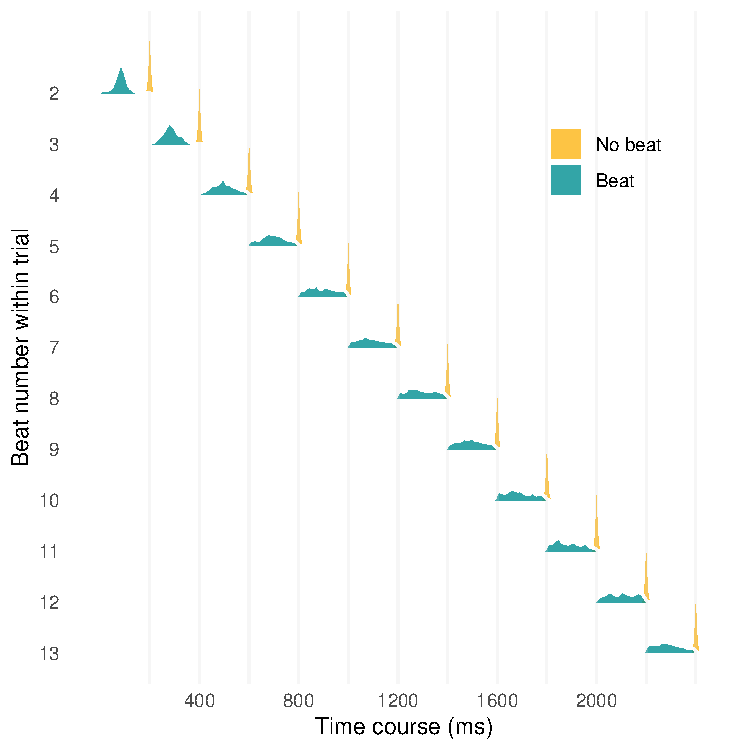
\includegraphics[width=\linewidth]{SP_24_visuals/Correct_and_Incorrect_distrubutions_by_beat_across_trial.pdf}
  \caption{Distribution of beats hit (space bar) over trials. Timing frames for each of beat (2-13) is illustrated by horizontal lines. No-beat distributions represent \cite{gorilla_Anwyl-Irvine_2019}'s measurement sensitivity}
  \label{fig:beat_data}
\end{figure}

For both Musical Ear tasks and each language task,  d-prime (d′) was calculated as a measure of sensitivity\cite{Macmillan_Creelman_2004}. For both auditory motor tasks, accuracy was calculating by averaging the percent of beats (rhythm) or pitches (melody) correct on each trial.


\setlength{\abovedisplayskip}{-10pt}
\setlength{\belowdisplayskip}{-10pt}
\setlength{\abovetopsep}{-10pt}
\setlength{\belowbottomsep}{-10pt}
\begin{table}[h]
\centering
\begin{tabular}{|c|c|c|}
\hline
\textbf{Task} & \textbf{Reported $\alpha$}& \textbf{Our $\alpha$} \\
\hline
GoldSmiths \cite{Müllensiefen_Gingras_Musil_Stewart_2014} & Range: 0.79 - 0.93 & 0.89 \\
Musical Ear tasks \cite{Wallentin_Nielsen_Friis-Olivarius_Vuust_Vuust_2010}& 0.87 & 0.79 \\
Auditory-motor melody \cite{Kachlicka_Saito_Tierney_2019}& Unreported & 0.93 \\
Auditory-motor rhythm\cite{Kachlicka_Saito_Tierney_2019}& Unreported & 0.91 \\
\hline
\end{tabular}
\caption{Task reported Cronbach's alpha values and our Cronbach's alpha values}
\label{tab:comparison}
\end{table}

\vspace{-\baselineskip}

\subsubsection{Statistical Analysis}

All quantitative variables from each of the tasks were centered on their mean to 0 and scaled across tasks, as seen in Figure \ref{fig:centered_data}. The Goldsmiths General scores were also discretized into categories based on three ranges, where score is: \text{Basic: } $<$ 36.1, \quad \text{Average: } $<$ 51.4 \text{ and } \geq 36.1, \quad \text{Higher than average: } \geq 51.4 \cite{Müllensiefen_Gingras_Musil_Stewart_2014}. 

\begin{figure*}[t]
  \centering
  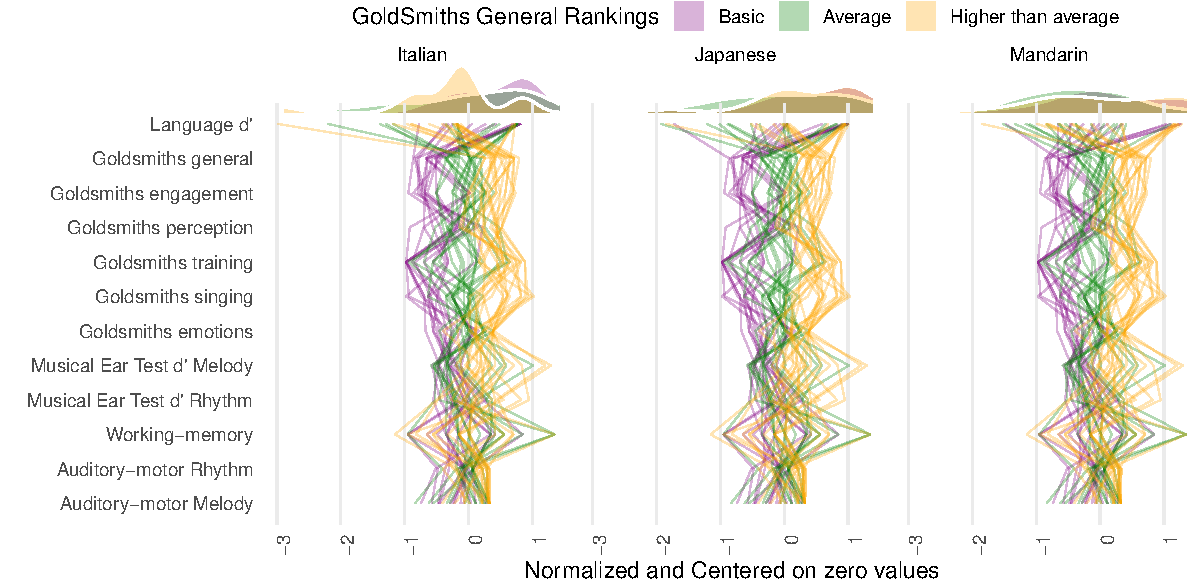
\includegraphics[width=.9\textwidth]{SP_24_visuals/by_gs.pdf}
  \caption{Raw data}
  \label{fig:centered_data}
\end{figure*}

To answer our three research questions, three multiple linear regression models (one per language) were built to compare the relative contribution of each task on centered and scaled d-prime scores of each language. Maximal models were built using the \textit{lm} package \cite{lmPackage} in R \cite{RManual}. Each model included 10 predictor effects: Goldsmiths engagement, Goldsmiths perception, Goldsmiths training, Goldsmiths singing, Goldsmiths emotions, Musical Ear Test d' Melody, Musical Ear Test d' Rhythm, Working-memory, Auditory-motor Rhythm, Auditory-motor Melody. Models were reduced in the following order: removal of non theoretical driven music skill (e.g., rhythm for Mandarin and Melody for Italian and Japanese), then effects were removed based on how much variance was explained in terms of coefficients and post hoc colinearity checks. The Japanese model was reduced minimally due to finding early evidence of parsimonious models. For Italian and Mandarin, the models were reduced to single variables for each theoretically driven question (e.g., music skill, music background) to achieve parsimony and reduce un-needed complexity. 

\section{Results}
Results from the Italian linear model found significant effects for: GoldSmiths emotions ($\beta$ = \livedata{modelsouts}{Italian.gs_emotions.estimate}, \text{SE} = \livedata{modelsouts}{Italian.gs_emotions.std.error}, z = \livedata{modelsouts}{Italian.gs_emotions.statistic}, p \textless{} \livedata{modelsouts}{Italian.gs_emotions.p.value}), indicating that higher musical emotional ratings predict lower sensitivity to Italian geminate contrasts; Working memory ($\beta$ = \livedata{modelsouts}{Italian.mean_working_memory.estimate}, \text{SE} = \livedata{modelsouts}{Italian.mean_working_memory.std.error}, z = \livedata{modelsouts}{Italian.mean_working_memory.statistic}, p \textless{} \livedata{modelsouts}{Italian.mean_working_memory.p.value}), indicating that higher working memory capacity predicts better ability to attenuate to sensitivity needed for Italian geminate contrasts.

Results from the Japanese linear model found significant effects for: GoldSmiths active engagement ($\beta$ = \livedata{modelsouts}{Japanese.gs_activeeng.estimate}, \text{SE} = \livedata{modelsouts}{Japanese.gs_activeeng.std.error}, z = \livedata{modelsouts}{Japanese.gs_activeeng.statistic}, p \textless{} \livedata{modelsouts}{Japanese.gs_activeeng.p.value}), indicating that higher amounts of musical engagement predict lower sensitivity to Japanese geminate contrasts; Working memory ($\beta$ = \livedata{modelsouts}{Japanese.mean_working_memory.estimate}, \text{SE} = \livedata{modelsouts}{Japanese.mean_working_memory.std.error}, z = \livedata{modelsouts}{Japanese.mean_working_memory.statistic}, p \textless{} \livedata{modelsouts}{Japanese.mean_working_memory.p.value}), indicating that higher working memory capacity predicts better ability to attenuate to sensitivity needed for Japanese geminate contrasts;
Auditory-motor Rhythm ($\beta$ = \livedata{modelsouts}{Japanese.beat_score.estimate}, \text{SE} = \livedata{modelsouts}{Japanese.beat_score.std.error}, z = \livedata{modelsouts}{Japanese.beat_score.statistic}, p \textless{} \livedata{modelsouts}{Japanese.beat_score.p.value}), indicating that higher productive rhythmic ability predicts greater sensitivity to Japanese geminate contrasts.

Results from the Mandarin linear model found significant effects for: GoldSmiths emotions ($\beta$ = \livedata{modelsouts}{Mandarin.gs_emotions.estimate}, \text{SE} = \livedata{modelsouts}{Mandarin.gs_emotions.std.error}, z = \livedata{modelsouts}{Mandarin.gs_emotions.statistic}, p \textless{} \livedata{modelsouts}{Mandarin.gs_emotions.p.value}), indicating that higher musical emotional ratings predict lower sensitivity to Mandarin tone; Musical Ear Test melody ($\beta$ = \livedata{modelsouts}{Mandarin.MET_dprime_melody.estimate}, \text{SE} = \livedata{modelsouts}{Mandarin.MET_dprime_melody.std.error}, z = \livedata{modelsouts}{Mandarin.MET_dprime_melody.statistic}, p \textless{} \livedata{modelsouts}{Mandarin.MET_dprime_melody.p.value}), indicating that higher perceptual sensitivity to musical pitch predicts higher sensitivity to Mandarin tone. 

Figure \ref{fig:model} plots the maximal model terms on the y-axis and coefficient estimates on the x-axis. The visualized estimate (point) and confidence interval (error bar) for each language indicates the results from the parsimonious model. In other words, if a term does not have a present co-efficient it means that it was not in the parsimonious model of that language.

\begin{figure}[t]
  \centering
  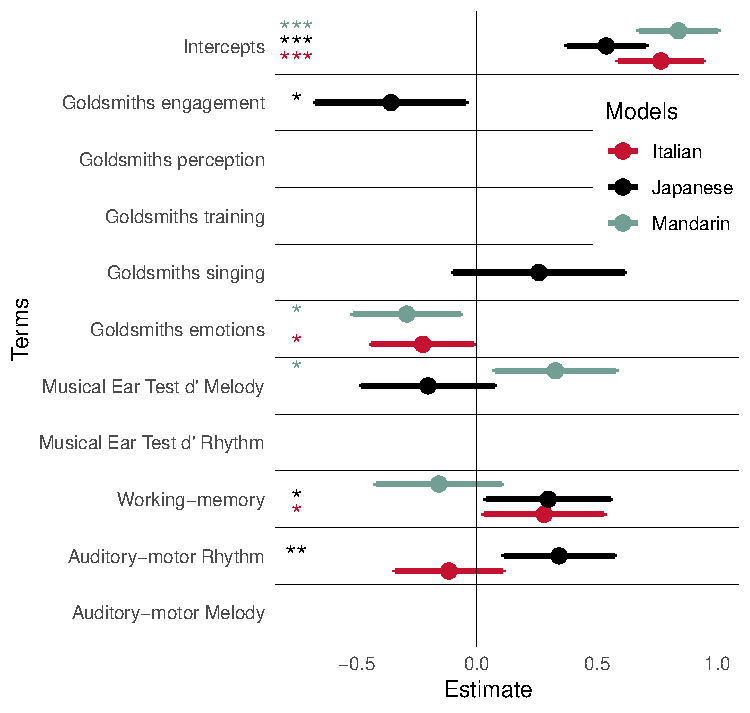
\includegraphics[width=\linewidth]{SP_24_visuals/Japanese,Italian,_Mandarin_max_models_structure:_parsimonious_effects.pdf}
  \caption{Each language's parsimonious model output}
  \label{fig:model}
\end{figure}

\section{Discussion}

The popular conjecture that musical ability is associated with improved language abilities is not a myth \cite{Slevc_Miyake_2006b}, however, the relationship is not as straightforward as the literature may suggest \cite{neves_et_al_2022_music}. With respect to our first research question, we found that musical pitch perceptual abilities do account for the most variance in terms of Mandarin tone sensitivity as previously reported in the literature \cite{zheng_et_al_2018_pitch}. Similarly, the Japanese model's results suggest that rhythm ability is indeed tied to Japanese geminate perception in line with previous theoretical claims \cite{lofqvist_2017_effect}. Interestingly, motor-auditory integration ability rather than perceptual ability is a superior predictor for sensitivity in Japanese geminate contrasts, while perceptual sensitivity to pitch better accounts for variance in Mandarin tone sensitivity, suggesting that different modalities of musical skill play differential roles across language cues. To the best of our knowledge, this is a new finding not reported in the previous music-to-language transfer literature. This is not to say, that the opposite modalities do not predict linguistic sensitivity, but rather that more variance is accounted for when using pitch-perception to predict Mandarin sensitivity and rhythm-production to predict Japanese sensitivity. Surprisingly, this effect does not carry over to the Italian task. It could be that the difference between Mandarin and Japanese model results have to do with how direct the relationship is between the linguistic cue and the musical cue. In the case of Mandarin tones and musical pitch, the same underlying cue of F0 is used to discriminate both whereas the relationship between geminate contrasts and music rhythm is less clear. Although both rhythm and geminate contrasts use duration cues, music rhythm, in our tasks, is measured as the ability to attenuate to the time between beats or the inter-beat interval, while geminate contrasts often rely on the duration of a consonant. In the case of Italian, it could be that no relationship between rhythm and language sensitivity was found because of the changes in vocalic pronunciation between geminate and non-geminate contrasts (co-articulation) \cite{Tsukada_Cox_Hajek_Hirata_2017}. In this way, it could be that Italian sensitivity would be better predicted by a person's ability to discriminate or produce formant differences. 

In terms of research question 2, Table~\ref{tab:comparison} shows that our methods of assessing music ability were reliable. Yet, while specialized skills in music are indeed positively predictive of non-native speech sensitivity, musical self-reported measures have the opposite effect. That is, in all cases throughout the models of each language, higher Goldsmith music sophistication scores predicted \emph{lower} non-native speech sensitivity. As seen in figure \ref{fig:centered_data} and corroborated by a post-hoc correlation matrix (see additional OSF materials), Goldsmiths score are highly correlated. This unexpected finding could be due to our specific population of university students, the propensity to over estimate ones music ability, or a more general finding that self-reported music ability is not directly associated with any foreign-language ability \cite{larrouy_maestri_et_al_2023_selfevaluation,correia_et_al_2023_selfawareness,schellenberg_et_al_2023_musical}. We tentatively conclude that while our exploratory results do suggest that higher music self ratings predict lower language sensitivity, further research is needed to clarify this finding. 

Lastly, with respect to research question 3, both the Japanese and Italian model suggest that working memory is a crucial predictor for sensitivity to geminate contrasts. This finding corroborates recent work that demonstrated how working memory can modulate non-native speech category learning success \cite{mchaney_et_al_2021_workingmemory}. Oddly, however, the Mandarin model did not find an effect of working memory. This could be because Mandarin words in our task are single syllable words based on one syllable, and Japanese and Italian words are varied multi-syllable words. \cite{mchaney_et_al_2021_workingmemory} used 5 different Mandarin syllables and found an effect of working memory. This result could also be due to the dimensionality of tone and geminate contrasts. Unlike tone, which has continuous cues for discrimination throughout a word, geminate contrasts happen only in limited segments of Japanese and Italian words. This could mean that partial information in the Mandarin task is sufficient, but higher cognitive demand is necessary for the Japanese and Italian tasks. Regardless, we conclude that domain general cognitive abilities like working memory play a crucial role in speech perception, particularly in the discrimination of non-native prosody, e.g., \cite{Kachlicka_Saito_Tierney_2019}

\section{Conclusions}

Our findings indicate that the relationship between music skills, cognitive abilities, and language skills is complex and demands continued investigations. We found that some measures of perceptual musical ability and working memory do, in fact, predict sensitivity to non-native speech whereas other measures, particularly productive musical ability, do not. We also observed unexpected findings in which higher self-rated music abilities predicted weaker sensitivity to non-native speech. Taken together, we call for a more nuanced approach to measuring and assessing music abilities and testing a more varied population of language users and musicians across different linguistic and musical stimuli.

\section{Acknowledgements}

This work was supported by the following grants: XXXX. We thank the instructors that allowed us to recruit in their classes and Kimiko Tsukada and colleagues for sharing their stimuli.

\bibliographystyle{IEEEtran}
\bibliography{my_references.bib}
\end{document}
